% ----------------------------------------------------
%   Burden and DeCrescenzo: Does the gender gap help the Democrats?
% ----------------------------------------------------


\documentclass[12pt
               ,final
               ]{article}



% --- Typeface, text, math, character encoding -----------------------
\usepackage{microtype}

% minion pro loads textcomp, McSymbol, amsmath
% if you want to pass options, load them beforehand
\usepackage{amsmath}
\usepackage[lf, mathtabular, minionint]{MinionPro} % serif familiy
\usepackage{MyriadPro} % sans-serif family
\usepackage[varqu, scaled = 0.95]{zi4} % mono w/ straight quotes


% \usepackage{mathptmx} % times with math font
% \usepackage{helvet} %sans fonts as helvetica clone
\usepackage[utf8]{inputenc}
\usepackage[T1]{fontenc}



% ----------------------------------------------------
%   REFERENCES
% ----------------------------------------------------
\usepackage{natbib}
 \bibpunct[: ]{(}{)}{;}{a}{}{,}
 \setlength{\bibsep}{0.0pt}
%\usepackage[nottoc,numbib]{tocbibind} % numbers the bibliography in the table of contents


% ----------------------------------------------------
%   MARGINS AND SPACING
% ----------------------------------------------------
\usepackage[margin=1in]{geometry} %margins % ipad geometry is 4X3
\usepackage{setspace}



% ----------------------------------------------------
%   TABLES AND FIGURES
% ----------------------------------------------------
\usepackage{graphicx} % input graphics
% \usepackage{float} % H float parameter
\usepackage{placeins} % \FloatBarrier function
\usepackage{rotating}
\usepackage{tikz}
\usetikzlibrary{shapes, positioning, matrix}

% % Define block styles
% \tikzstyle{decision} = [diamond, draw, fill=blue!20, 
%     text width=4.5em, text badly centered, node distance=3cm, inner sep=0pt]
% \tikzstyle{block} = [rectangle, text centered, rounded corners, minimum height=4em]
% % \tikzstyle{line} = [draw, -latex']
% \tikzstyle{cloud} = [draw, ellipse,fill=red!20, node distance=3cm,
%     minimum height=2em]

% \usepackage{qtree}

% table packages removed! we don't have any tables!




\usepackage{hyperref}
\hypersetup{colorlinks = true, 
            citecolor = black, 
            linkcolor = violet, 
            urlcolor = teal}

% todo notes
\usepackage[colorinlistoftodos, 
            prependcaption, 
            obeyFinal,
            textsize = footnotesize]{todonotes}
 \presetkeys{todonotes}{color = violet!30}{}
\usepackage{comment}

% spacing and other formatting
\usepackage{enumitem} % allows nosep command for lists
  \setlist{noitemsep} % (no separation between list items)




% \usepackage{sectsty} % section styles
%   \allsectionsfont{\raggedright \rm}
%   \sectionfont{\sc}

\usepackage[rm, small, sc]{titlesec}
\titleformat*{\subsection}{\itshape}
\titleformat*{\paragraph}{\itshape}



% abstract tweaks given sectsty formatting things?
\usepackage{abstract}
\renewcommand{\abstractname}{\sc Abstract}    % clear the title


% ----------------------------------------------------
%   Tikz
% ----------------------------------------------------
\usepackage{tikz}
  \tikzstyle{entry} = [minimum width=0.5in, minimum height=0.25in, text centered]
  \tikzstyle{arrow} = [thick,->,>=stealth]


% ----------------------------------------------------
%   USER COMMANDS
% ----------------------------------------------------
\newcommand{\notes}[1]{\\
% \raggedright 
\small
\emph{Notes:} #1}





% ----------------------------------------------------
%   BEGIN
% ----------------------------------------------------

\begin{document}

\title{Mobilization, Persuasion, and the Partisan Fallout of the Gender Gap in U.S.\ Voting%
  \thanks{We thank Luis Fraga, Devin Judge-Lord, Ryan Moore, Paul Testa, and participants at the American Politics Workshop at the University of Wisconsin-Madison, the 2016 Toronto Political Behavior Workshop, and the 2017 meeting of the Midwest Political Science Association for comments on earlier drafts of this paper. Authors are listed alphabetically.}
}

\author{}
\author{Barry C.\ Burden\footnote{Professor of Political Science, University of Wisconsin--Madison (\url{bcburden@wisc.edu})} 
\and 
Michael G.\ DeCrescenzo\footnote{Graduate Student, University of Wisconsin--Madison (\url{decrescenzo@wisc.edu})}}

\date{Updated \today}
\maketitle

\todo[inline]{Tikz flowcharts}



\hypersetup{pageanchor=false}
\thispagestyle{empty}




\listoftodos


% \vspace{11cm}





% ----------------------------------------------------
% ----------------------------------------------------


\newpage


\thispagestyle{empty}





\begin{abstract} 

% rewrote this aug 21, 2018 (MGD)
Does the gender gap help the Democrats? To answer this question, we provide a theoretical framework to understand how group differences in voting affect party vote shares. We apply this method to the gender gap in U.S. voting. Our approach views both the gender gap and the election outcome as underlying partisan predispositions in the electorate that are transformed through partisan mobilization, partisan defection, and the choices of unaffiliated voters. We argue that the size of the gender gap has no necessary bearing on the partisan vote outcome. Rather, the relationship is contingent on the changing numerical impact of partisanship, partisan mobilization, and persuasion over time. Although the gender gap and the Democratic vote in presidential elections have both increased since over several decades, this relationship is spurious. The primary cause of the gender gap (partisan change) was actually harmful to the Democrats. Meanwhile, forces that increased the Democratic vote (mobilization and persuasion) were minor influences on the gender gap. Our framework can be extended to understand how other group cleavages affect election outcomes.

% Does the gender gap help the Democrats? To answer this question, we provide a generalizable theoretical framework to understand the link between group differences in vote choice, turnout, and party vote shares, with an application to the gender gap. Our methodological approach views both the gender gap and partisan election outcomes as underlying partisan predispositions in the electorate that are transformed through partisan mobilization, partisan defection, and the choices of unaffiliated voters. We provide a strategy for measuring the effects of these forces on a common scale. We argue that the size of the gender gap has no necessary bearing on the partisan vote outcome. Rather, the relationship is contingent on how the mobilization of party supporters and the persuasion of nonsupporters translate partisan predispositions into votes. Although the gender gap and the Democratic vote in presidential elections have both increased over time, we demonstrate that the primary cause of the gender gap (partisan change) was actually harmful to the Democrats. Meanwhile, forces that increased the Democratic vote (mobilization and persuasion) were minor influences on the gender gap. Our framework can be extended to understand how other group cleavages affect election outcomes.

\end{abstract}


\hfill
\begin{center}
  Keywords: gender gap, voting, mobilization, voter persuasion, party identification
\end{center}

\todo[inline]{Gap in party ID that appeared early but was suppressed by unequal mobilization and persuasion}

\todo[inline]{theoretical/necessary relationship vs empirical/contingent relationship (in the theory section)} 


\todo[inline]{We say ``no general relationship'' between the gender gap and the Democratic vote, but maybe that isn't true. If partisanship is the leading influence on the gap, then the leading effect of the gap is negative. Since mobilization and persuasion affect the vote, but not ``through'' the gap, then we shouldn't attribute that as an ``offsetting'' effect on the gap. The topline relationship is positive, but that is spurious. The true relationship (controlling away the spuriousness) is negative.}






% ----------------------------------------------------
% ----------------------------------------------------





\newpage

\hypersetup{pageanchor = true}
\pagenumbering{arabic}

\doublespacing

The disparity in the vote choices of men and women has risen to a double digit gap in recent U.S.\ national elections and has generated much analysis and discussion by the public, journalists, campaigns strategists, and academic researchers. Although the votes of men and women are not as divergent as other notable groups in the electorate, the gender gap is uniquely consequential for American elections because the two groups in question are nearly equal in size. Small shifts in the voting behavior of either men or women would have acute electoral effects. In this paper we seek to understand how the size of the gender gap influences election outcomes.

% cuts cites to Norrander, Wirls, gap figure

We ask two questions about the gender gap in U.S.\ voting. First, does a larger gender gap advantage the Democratic Party? Although journalists and pundits often presume that a larger gender gap implies that Democratic candidates have earned more votes from women \citep{kaufmann1999changing}, we are unaware of any evidence that a larger gender gap creates a numerical advantage for either party. The gender gap, conventionally defined as the percent of women voting Democratic minus the percent of men voting Democratic, can fluctuate for several reasons. Women may vote more highly Democratic, but men may also vote more highly Republican. Moreover, these gender differences may be driven by long-term partisan change or short-term variation in voter turnout and swing voting. As a result, the effect of the gender gap on the Democratic vote is unclear without a model to describe the processes that create the gap. This is the focus of our second question. To the extent that the gender gap and the Democratic vote are linked, what balance of long and short-term mechanisms shape postwar electoral outcomes?

To answer these questions, we develop a general theory and an empirical approach to describe how voting gaps between groups in the electorate can advantage one party over another. Theoretically, we show that voting gaps and election outcomes are the result of the same underlying process: partisan preferences act as a baseline for election outcomes, but partisanship is transformed into votes through the mobilization of same-party supporters, swing voting by other-party supporters, and the votes of the party-unaffiliated. 
% the goal here is to lay out the 4 pieces in one solid overture
By conceptualizing elections and group-level voting under the same framework, we can directly compare the partisan impact of partisanship, mobilization, and persuasion among men and women over time. Methodologically, we use simple math to measure these mechanisms in the electorate on a common scale, which existing measures fail to do. We apply our method to survey data from 17 presidential elections (1952--2016) to decompose the sources of the two parties' votes: how much of the vote is attributable to partisanship, mobilization, persuasion, and independents, and where do gender differences in these mechanisms emerge?

% Theoretically, we argue that election results are the end result of a process that starts with underlying partisan preferences in the electorate; these long-term predispositions are altered in each election by differential turnout and crossover voting. These processes may shape the votes of men and women (or other groups) in different ways, and their impact on elections can change over time. Methodologically, we devise a strategy for measuring these processes on a common scale to determine their impact on the gender gap and the final vote using simple math to compute each. Using survey data over 16 presidential elections (1952--2012), we decompose the parties' votes to trace how patterns in mobilization and persuasion, plus votes of the unaffiliated, among men and women create both the gender gap and the Democratic vote share.

\todo[inline]{Concern about formalization: is there a way to look at derivatives or variance decomposition in the data to determine, formally, the ``effect'' of each process as a mathematical statement? Next paper?}

Our study delivers a key insight about the relationship between the gender gap and the Democratic vote share: the forces driving over-time variation in the gender gap are not the same forces that drive over-time variation in the Democratic vote. The gender gap initially emerged from a long-term increase in Republican partisanship among men from the 1960s through the 1980s, which negatively affected the Democratic vote. 
% caveat about recent partisanship among women?:
% In the years since the initial onset of the gender gap, fluctuation in women's partisanship has affected the gender gap in the short-term, but the impact and permanence is dwarfed by the partisan drift among men.
During roughly the same time period, the Democratic Party's historical disadvantages in partisan mobilization and partisan defections narrowed, boosting the Democratic vote share but in a relatively gender-neutral way. 
% Unaffiliated voters contribute to election outcomes in important ways, but aggregate voting differences between Independent men and Independent women were also small compared to the large effects of partisan change. 

\todo[inline]{Independents are growing but not affecting the gender gap}

This article has important contributions for the study of partisan coalitions as well. Our approach can be applied to various group cleavages in voting, including racial and ethnic groups, college and non-college educated citizens, the working and non-working classes, and urban and rural residents. As political parties compete to build winning coalitions, they attract certain voters while repelling other voters. Our method exposes these trade-offs in the parties' strategies by comparing the electoral impact of partisanship, mobilization, and persuasion on the same scale. 

% deleted note about ``two eras'' of gender gap
% era 1: compounding harm to democrats
% era 2: short-term fluctuation that can help the Democrats sometimes but probably won't grow permanently

% do we have a ``our contributions are [blank]'' way of putting this?



\section*{Does the Gender Gap Help the Democrats?}
\label{sec:topline}

\todo[inline]{Combine w/ next section? First, there is no such relationship. Second, we question whether there should be one.}

In their coverage of recent elections, journalists and pundits often argue that Democrats are more successful at the ballot box when the votes of men and women diverge.\footnote{For now we set aside the concern about casting men and women as monolithic voting blocs. Our approach does allow for men and women to differ in their turnout rates and how much they vote against their party affiliations.} For example, in the run up to the 2012 presidential election, the \emph{Washington Post} reported that ``The Republicans are on the defensive partly because the gender gap---in which Democrats have a sizable advantage among women---is growing.''%
 \footnote{Robert McCartney, ``Romney's Woes Threaten McDonnell and Allen,'' \textit{Washington Post}. October 7, 2012.}
Commentary on the Democratic Party's demographic coalition frequently identifies women as a crucial but unsteady constituency, thus framing the gender gap as a function of women's voting rather than men's. Writers often describe Democrats' liberal positions on issues of feminism and women's role in society as ``a line of attack that has generated a gender gap and has been crucial to past Democratic victories,'' while Republicans are victorious when they can effectively counter accusations of a ``war on women,'' as they did in the 2014 midterm elections.%
 \footnote{Thomas B. Edsall, ``Making the President Small,'' \textit{The New York Times}, November 5, 2014.}
Another report in \textit{USA Today} on the eve of the Republicans' triumph in the 2010 midterm elections observed that ``men generally tilt toward GOP candidates, so a significant narrowing of the gender gap among women is contributing to Democrats' struggles,'' concluding that Democrats would only win ``by mobilizing women voters.''%
 \footnote{Mimi Hall, ``Democrats Lose Share of Women to GOP,'' \textit{USA Today}, October 20, 2010.}

This conventional wisdom occasionally appears in academic scholarship as well. Studies of party coalitions occasionally interpret the Democrats' reliance on women's votes as an advantage over Republicans. For instance, \citet{zingher2014analysis} finds that greater mobilization among Democratic women increased their contribution to the Democratic electoral coalition in recent decades, while men's contribution to the Republican coalition has been largely unchanged over the same period, implying that divergent voting among men and women over time bolsters the Democratic coalition on net. Others concur that Democrats' ``marginal support'' among women has been increasing since the 1960s \citep{stanley1986partisanship} and that ``Attracting women\ldots remained a problem'' for Republican efforts to rebuild their electoral coalition in the 1990s and 2000s \citep{stanley2006partisanship}. Scholarship on the gender gap itself, on the other hand, finds that women's rising prominence in the Democratic coalition is matched or even superceded by increasing Republican partisanship among men (e.g.\ \citealt{kaufmann1999changing}), so different literatures have different interpretations of the relationship between the gender gap and the Democratic vote. 

\begin{figure}[hbt]
  \centering
  \caption{The Gender Gap and the Presidential Vote}
  \includegraphics[width = \textwidth]{graphics/topline-3-panel.pdf}
  \label{fig:topline}
  \notes{Plots contain correlation coefficients (labeled ``r''), regression coefficients (``b''), coefficient standard errors (``se''), and $p$-values (``p''). Exit poll data were obtained from CNN and include Washington D.C.\ as a state. Election results from U.S.\ Election Atlas.}
\end{figure}

Before introducing our approach, we provide evidence that there is no simple relationship between the gender gap and the Democratic vote.
First, we analyze the relationship using national data from 1952 through 2012.%
  \footnote{Data from 2016 are not yet included in the cumulative data file. We elect not to use the 2016 cross-sectional file in case the sample weights diverge from the sample weights that will eventually be included in the cumulative file.}
This approach covers a wide range of elections from landslides such as 1972 to nail-biters such as 2000. The dependent variable is the official percentage of the two-party popular vote won by the Democratic ticket. We calculate the gender gap as the Democratic share of the two-party vote among women minus the Democratic share among men using the American National Election Studies cumulative data file. The first panel of Figure~\ref{fig:topline} displays the data with an OLS regression line, the 95 percent confidence interval, and statistics to characterize the estimated relationship. There is little sign of a meaningful relationship, as the correlation is low and the $p$-value is high. A second way to evaluate the relationship is cross-sectionally, using state level data from individual elections. For this cross-sectional test, we calculate the gender gap from exit poll data for the 50 states and Washington D.C.\ from the 2004 and 2008 presidential elections.%
  \footnote{More recent data would also be useful, but exit polls excluded 19 states in 2012 and 22 states in 2016.} 
We again compute the Democratic share of the two-party vote as the outcome of interest, this time using official state-level results. The state-level data appear in the second and third panels. The cross-sectional data tell the same story as the longitudinal analysis. There is little sign of a meaningful relationship, as evidenced by the weak and insignificant correlations and regression slopes. 

Taking these two tests together, we find little evidence of a positive relationship between the gender gap and the Democratic vote. However, there are theoretical grounds for questioning this superficial evidence. The gender gap as commonly measured is useful as a comparison of vote choices by gender, but it says nothing about how many votes the gap is ``worth'' for each major party candidate. Uncovering the partisan impact of the gender gap requires more theoretical and empirical care.

\FloatBarrier
\section*{From Party ID to the Vote: Mobilization and Persuasion}
\label{sec:define-mob-per}

% dropped the PID graphic and associated text

Popular wisdom suggests that Democrats are advantaged when the gender gap is wider, but the precise explanation for this is not obvious. Writers sometimes suggest that the key mechanism linking the gender gap and the Democratic vote is the underlying differences in the party loyalties of men and (especially) women, while other reports suggest that gender differences turnout or swing voting are the main drivers. We argue that each of these electoral forces---partisanship, mobilization, and persuasion---are potentially important, but they would distinct effects on the gender gap and the Democratic vote that are important to decompose. Moreover, these mechanisms are not directly comparable using conventional measures, so we require a new approach to answer the question at hand.

Research on the relationship between party ID and the gender gap challenges the view that the gap helps Democrats. Numerous authors have shown that the gender gap first emerged due to changing partisan inclinations of \emph{men} rather than women \citep{kaufmann1999changing,norrander1999evolution,wirls1986reinterpreting}. They document that men's partisan attachments grew more Republican through the 1970s and 80s while women's partisanship remained relatively stable. If the gender gap is the result of Republican shifts among men, then Democrats actually would be quite harmed by the arrival of the gender gap. 

Although the gender gap in party identification provides important raw material to form the gender gap in voting, the two are not the same. \citet{kaufmann1999changing} and \citet{chaney1998explaining} find that party ID often accounts for less than half of the voting gap. We argue that the gap observed in voting must be related to party ID in the larger electorate, but it also must be filtered in two primary ways. The two parts of this filtering function are (1) how many partisan men and women turn out to vote for their preferred parties (the \emph{mobilization} effect) and (2) how many partisan men and women defect to vote for the opposing party (the \emph{persuasion} effect).%
  \footnote{In addition, the votes of unaffiliated voters may contribute the outcome in a gendered fashion. We incorporate these voters when we describe the empirical approach.}

We discuss persuasion first because it is the more intuitive mechanism. In any election, some Democratic partisans vote for the Republican candidate, and some Republican partisans vote for the Democratic candidate. If the Democratic candidate earns more crossover votes than the Republican candidate does, we can describe persuasion as a net benefit to Democrats. In turn, if Democrats earn more votes on net from Republican \emph{women} than Republicans net from defections among Democratic \emph{men}, then gender differences in persuasion are also a net benefit to Democrats' bottom-line vote shares. Although this relationship appears almost tautological, it is more contingent than it seems. For one, the net effects of persuasion depend on the underlying distribution of party ID among men and women. Because the sizes of the partisan bases are not equal nor constant across time, comparing the defection \emph{rates} for each party will not capture the real vote impact of partisan defection. Moreover, the parties' relative successes in persuasion may be related to their advantages in other mechanisms. For example, short-term electoral context favoring one party may lead to high levels of swing voting, but it may also drive a concomitant turnout increase for the advantaged party and a decrease for the disadvantaged party, obscuring the overall value of persuasion. The framework and method we develop below allow for all of these influences to act simultaneously.

The potential connection between mobilization and the gender gap is more complex. Consider a scenario in which the short-term electoral context favors the Democratic Party. Democrats, who are more likely to be women, are more enthusiastic than Republicans and thus vote at higher rates. This could increase the correlation between the gender gap and the Democratic vote by boosting the overall level of Democratic voting among women in particular. Lower enthusiasm among Republicans may decrease this correlation however, because lower turnout among Republicans would lead the partisan distribution among men voters to shift in the Democratic direction. By contrast, electoral contexts that favor the Republican party may increase enthusiasm among Republican-leaning men but decrease enthusiasm among Democratic women, so the Republican vote share may grow with unclear implications for the gender gap. The relationship between the gender gap and the Democratic vote would thus depend on which groups are most affected by the shifting electoral context. Campaign mobilization also targets voters in a gendered fashion with a more obvious implication for the gender gap and the Democratic vote. If Democratic efforts to ``get out the women's vote'' are successful, this should increase the correlation between the gender gap and the Democratic vote as long as mobilization of Democratic women is not offset one-to-one by counter-mobilization of Republican men. 

The various mechanisms that influence the gender gap are intertwined in ways that obscure their impact on the partisan electoral outcomes. Long-term shifts in party ID certainly coincide with the rise of the gender gap, but can changes in mobilization and persuasion. As men have become more Republican, women voters have grown as a share of the voting electorate, and party-loyal voting has reached monumental levels \citep{zingher2014analysis,bartels2000partisanship,bafumi2009new}. To make sense of these simultaneous trends, we require a theory to understand how group voting patterns and election outcomes are related, and we require a measurement method that compares each mechanism's contribution to the vote on a common scale. 



\section*{A Theory of Group Voting Gaps}
\label{sec:theory}

Much research on the gender gap examines where men and women's vote preferences come from in the first place: policy attitudes, economic circumstances, social position, partisan sorting, and other gender-specific experiences that may bear on one's personal political orientation \citep{box2004dynamics,chaney1998explaining,conover1988,edlund2002,gillionetal,kaufmann1999changing,manza1998gender}. Our purpose is not to revisit any of these insightful explanations for why men and women are attracted to different parties. Instead, we hope to unpack an important but blurred distinction between party identification and voting behavior. Party ID is a relatively stable and slow-moving attitude, whereas vote choice is a discrete action that also reflects short-term electoral context and campaign-specific dynamics.%
 \footnote{This insight is the basis of the Michigan school's classification of presidential elections as ``maintaining,'' ``deviating,'' or ``realigning'' \citep{campbell1966classification} and the development of the concept of the ``normal vote'' based on party ID \citep{converse1966normalvote,levendusky2008measuring}.}
Indeed, two major reasons why election results do not perfectly reflect the distribution of party identification in the electorate are that rates of turnout vary between the parties and because partisans engage in swing voting at different rates.

We develop a theoretical perspective to trace how partisan attachments are translated into votes through the dual processes of mobilization and persuasion. Our approach is designed to highlight (1) how gender differences in each of these mechanisms aggregate into the overall gender gap and (2) how many votes each party earns from men and women along the way. Although we focus on gender in this paper, our approach can be generally applied to many other consequential groups in recent elections, such racial and ethnic groups, college and non-college educated citizens, the working and non-working classes, or urban and rural residents. We believe that our theoretical foundation can be extended to study larger numbers of groups and more elaborate electoral systems.%
 \footnote{We acknowledge that gender is in fact more complex and contested than the binary classification of ``male'' and ``female'' suggests. However, these are the terms in which the gender gap has been defined and studied. In addition, those two categories are the only valid gender codes in the ANES cumulative file.}

% \todo[inline]{Include a parting note about potential for formalizing the results further?}

The gender gap is conventionally defined as the Democratic vote share among women minus the Democratic vote share among men.%
 \footnote{There are some alternatives. \citet{norris2003} computes the net partisanship of women minus the net partisanship of men.} 
This is how we measure the gap in the scatterplots presented earlier. However, because vote shares are proportions, and because vote proportions do not convey \emph{how many votes} they are worth, the size of the gender gap as conventionally defined does not contain enough information to determine which party benefits overall. Our approach is premised on first accounting for the \emph{raw number of votes} each party collects from each gender, and then decomposing these votes into the mechanisms of mobilization and persuasion (plus the votes of unaffiliated voters) to trace how many votes are produced by each process. This framework is reminiscent of \citet{axelrod1972votes}'s analysis of coalition composition (see also \citealt{stanley1986partisanship}), but goes further in important ways. Whereas Axelrod defines the groups within a party's coalition \emph{a priori} and examines the parties one a time, we examine group dynamics in both parties simultaneously and explicitly distinguish between votes earned by party supporters and by party non-supporters. We believe that this approach resembles how campaign strategists actually think about building winning coalitions by turning out supporters who have long-term attachments to the party (``getting out the vote'' or GOTV) and persuading supporters of the opposing party to cross over.% 
 \footnote{We acknowledge that in both real campaigns and political analysis it can be challenging and perhaps even artificial to separate partisanship, mobilization, and persuasion, although authors have tried (\citealt{huber2007identifying}). They are likely to be related, as when a campaign seeks to strengthen the partisans bonds of its supporters as a means to mobilize them and prevent defection to their opponents. But lines need to be drawn somewhere, and we believe that the explicit model we outline is transparent, defensible, and flexible enough to permit refinements in future studies.}

We now present a series of stylized illustrations to outline our approach, building upward from microfoundations to aggregate results. We formalize these illustrations into equations in the following section. To present the logic in a clear fashion, we temporarily ignore voters who are unaffiliated with either party; they will be incorporated in the empirical analysis. These illustrations should make clear that our methodological approach relies on simple math such as addition and percentages rather than regression modeling.

In the U.S.\ two-party system, every citizen must make one of three potential choices in the election: voting Democratic, voting Republican, or not voting.%
 \footnote{We begin by assuming only two parties (ignoring minor parties and independent candidates) for ease of exposition.} 
Assuming that voters have some baseline affiliation for one party, the raw number of votes for a party is the sum of (1) party supporters who have been mobilized to vote and (2) supporters of the other party who have been persuaded to switch sides in the current election. We refer to the number of votes one party earns over the other as \emph{net Democratic votes}. The flowchart below visualizes how the number of net Democratic votes in an election is the result of partisan mobilization and persuasion.
%
 % \begin{center}
 %  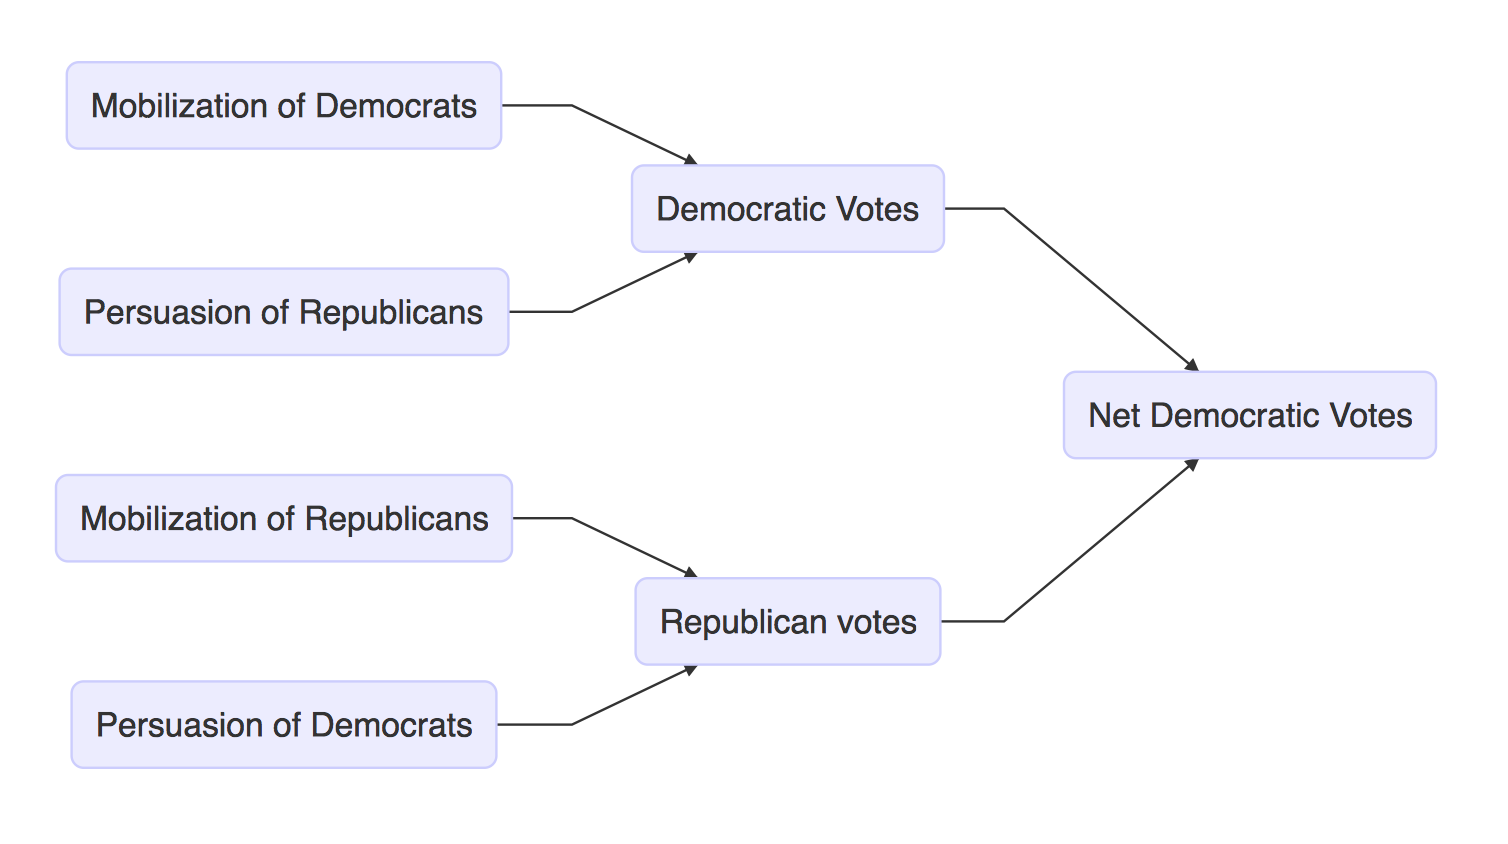
\includegraphics[width = 0.9\textwidth]{diagrams/net-votes.png}
 % \end{center}

\begin{center}
  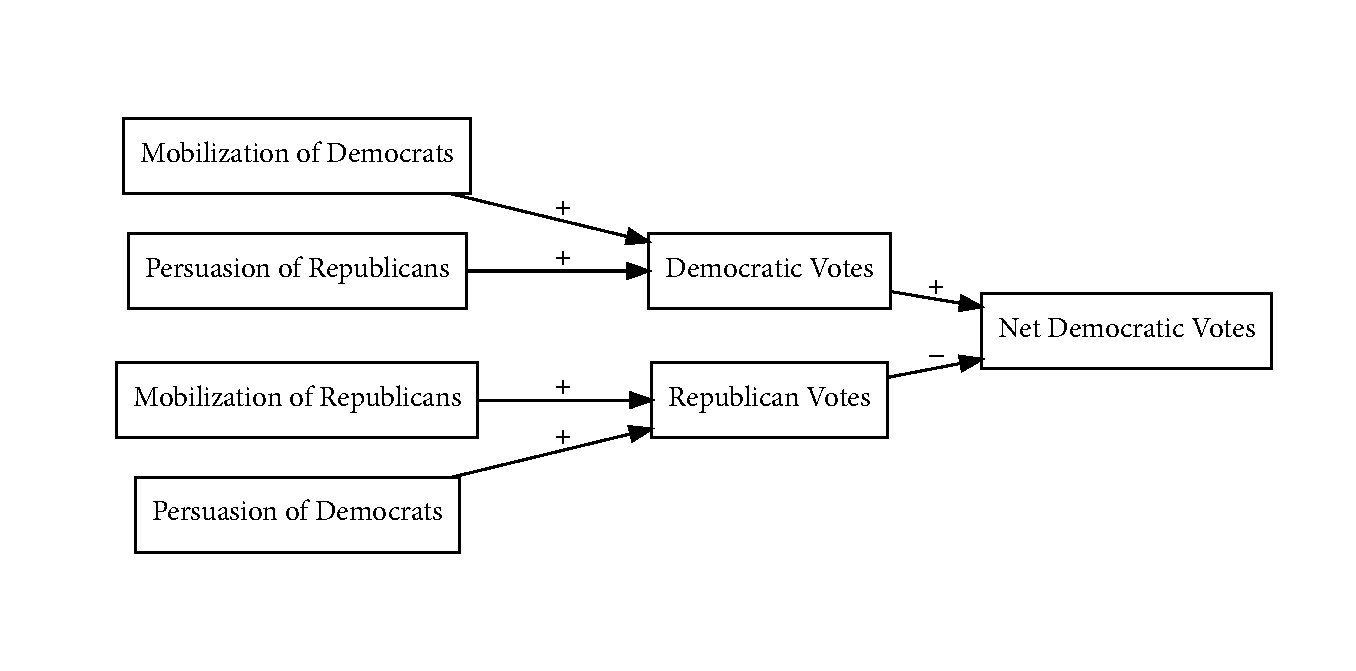
\includegraphics[width = \textwidth]{diagrams/net-votes.pdf}
\end{center}

% \noindent
% \begin{tikzpicture}
%   \matrix (m) [matrix of math nodes,
%                row sep = 1em, column sep = 4em, minimum width = 2em] {
%   \text{Mobilization of Democrats} \\
%   & \text{Democratic Votes} \\
%   \text{Persuasion of Republicans} \\
%   & & \text{Net Democratic Votes} \\
%   \text{Mobilization of Republicans} \\
%   & \text{Republican Votes} \\
%   \text{Persuasion of Democrats} \\
%   };
%   \path[-latex]
%     (m-1-1.east) edge node [above] {+} (m-2-2)
%     (m-3-1.east) edge node [above] {+} (m-2-2)
%     (m-5-1.east) edge node [above] {+} (m-6-2)
%     (m-7-1.east) edge node [above] {+} (m-6-2)
%     (m-2-2.east) edge node [above] {+} (m-4-3)
%     (m-6-2.east) edge node [above] {-} (m-4-3)
%       ;
% \end{tikzpicture}


The number of net Democratic votes differs from the conventional measure of two-party vote share, but it is advantageous because its components can be rearranged in several valuable ways. One such rearrangement incorporates the notion of \emph{net vote advantage} in mobilization and persuasion. The Democratic Party has a net advantage in mobilization if it earns a greater number of votes from loyal Democrats than the Republican Party earns from loyal Republicans. We can express the number of net Democratic votes as the sum of the Democrats' net advantages in mobilization and in persuasion. The core benefit of this approach is the ability to compare the effects of mobilization and persuasion on the same scale, which is impossible with typical measures that use different denominators. In cases where turnout and swing voting rates are similar between the parties, one party still has an advantage if it has a larger partisan base. Our approach handles these cases by accounting for the size of the partisan bases.
%
 % \begin{center}
 %  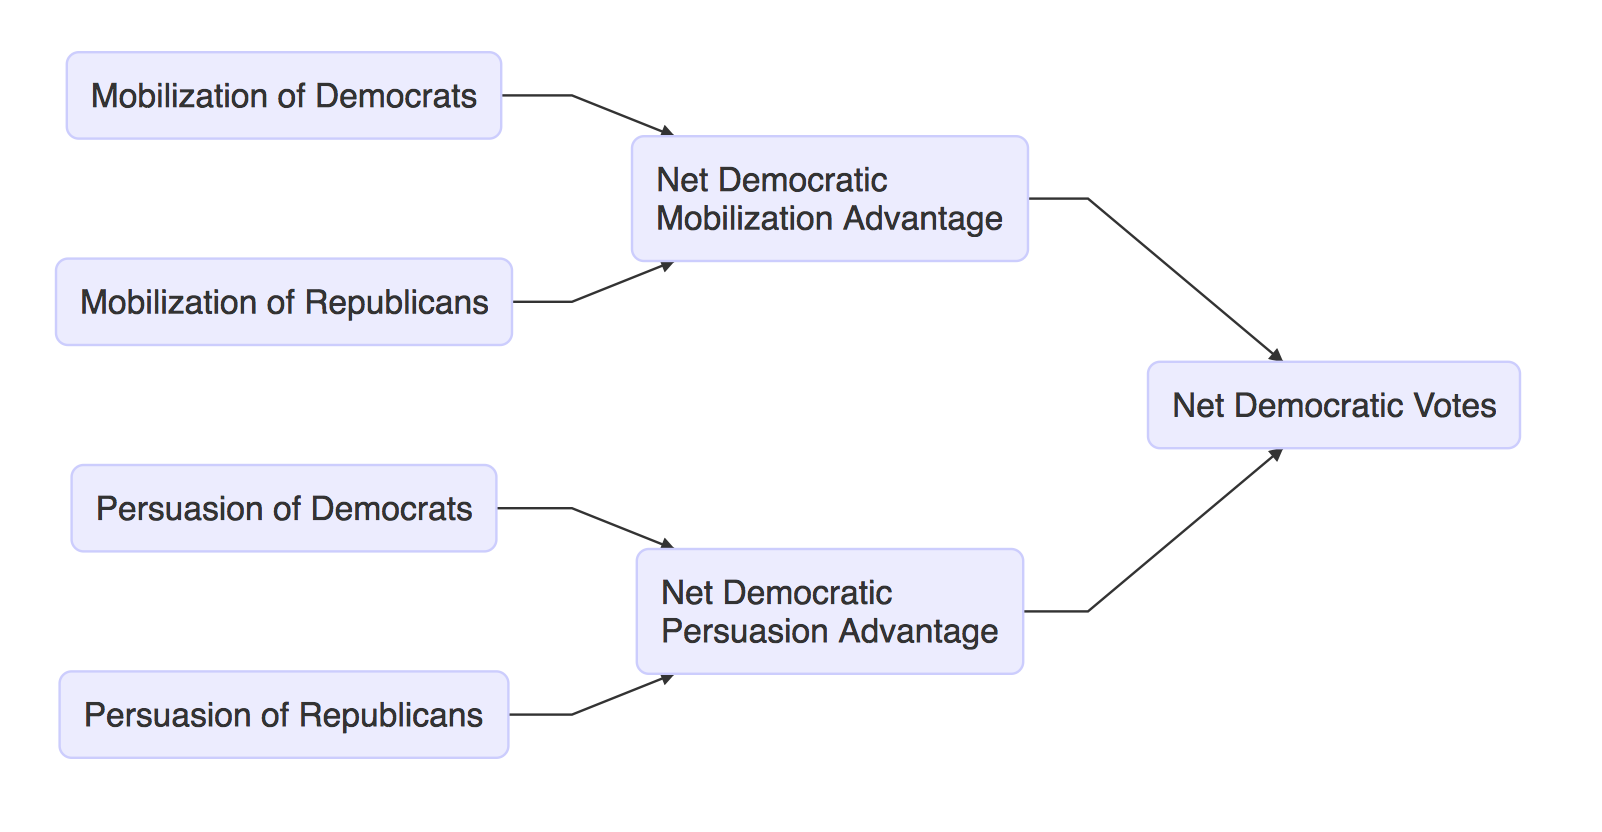
\includegraphics[width = 0.9\textwidth]{diagrams/net-votes-mechanisms.png}
 % \end{center}

\begin{center}
  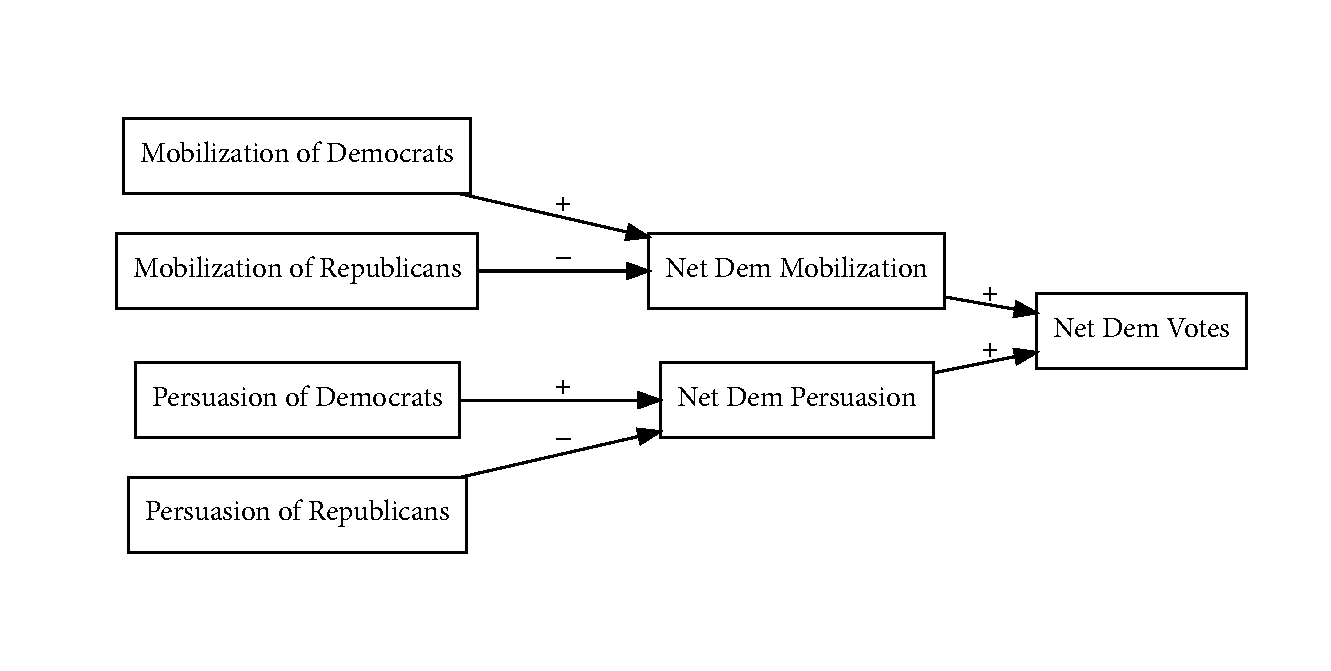
\includegraphics[width = \textwidth]{diagrams/net-vote-mechanisms.pdf}
\end{center}

% \noindent
%  \begin{tikzpicture}
%   \matrix (m) [matrix of math nodes,
%                row sep = 1em, column sep = 4em, minimum width = 2em] {
%   \text{Mobilization of Democrats} \\
%   & \text{Net Dem Mobilization} \\
%   \text{Mobilization of Republicans} \\
%   & & \text{Net Dem Votes} \\
%   \text{Persuasion of Democrats} \\
%   & \text{Net Dem Persuasion} \\
%   \text{Persuasion of Republicans} \\
%   };
%   \path[-latex]
%     (m-1-1.east) edge node [above] {+} (m-2-2)
%     (m-3-1.east) edge node [above] {-} (m-2-2)
%     (m-5-1.east) edge node [above] {+} (m-6-2)
%     (m-7-1.east) edge node [above] {-} (m-6-2)
%     (m-2-2.east) edge node [above] {+} (m-4-3)
%     (m-6-2.east) edge node [above] {+} (m-4-3)
%       ;
% \end{tikzpicture}

% keep this
% Beginning with votes rather than vote shares also allows us to straightforwardly decompose these mechanisms and net advantages by gender. As we argue above, the gender gap as it is typically measured does not include enough information to determine which party numerically benefits from gender differences in voting. 

% % By computing net Democratic votes separately for men and women, we can identify gender gaps in each mechanism and trace how these component gender gaps aggregate into the gender gap we observe in the final vote outcome. 

Our method allows us to measure the gender gap in terms of mobilization and persuasion as well. We call this new measure the \emph{net gender gap}: the number of net Democratic votes among women minus the net Democratic votes among men. As with the net Democratic vote, we can decompose the net gender gap into the separate mechanisms of mobilization and persuasion and measure the gender gap in each mechanism. This is done by calculating net Democratic advantages in mobilization and persuasion separately for men and women. If the net Democratic advantage in any mechanism is greater for women than men, the gender gap in that mechanism is positive. The net gender gap is thus the sum of the gender gap in each of these mechanisms. 

 % \begin{center}
 %  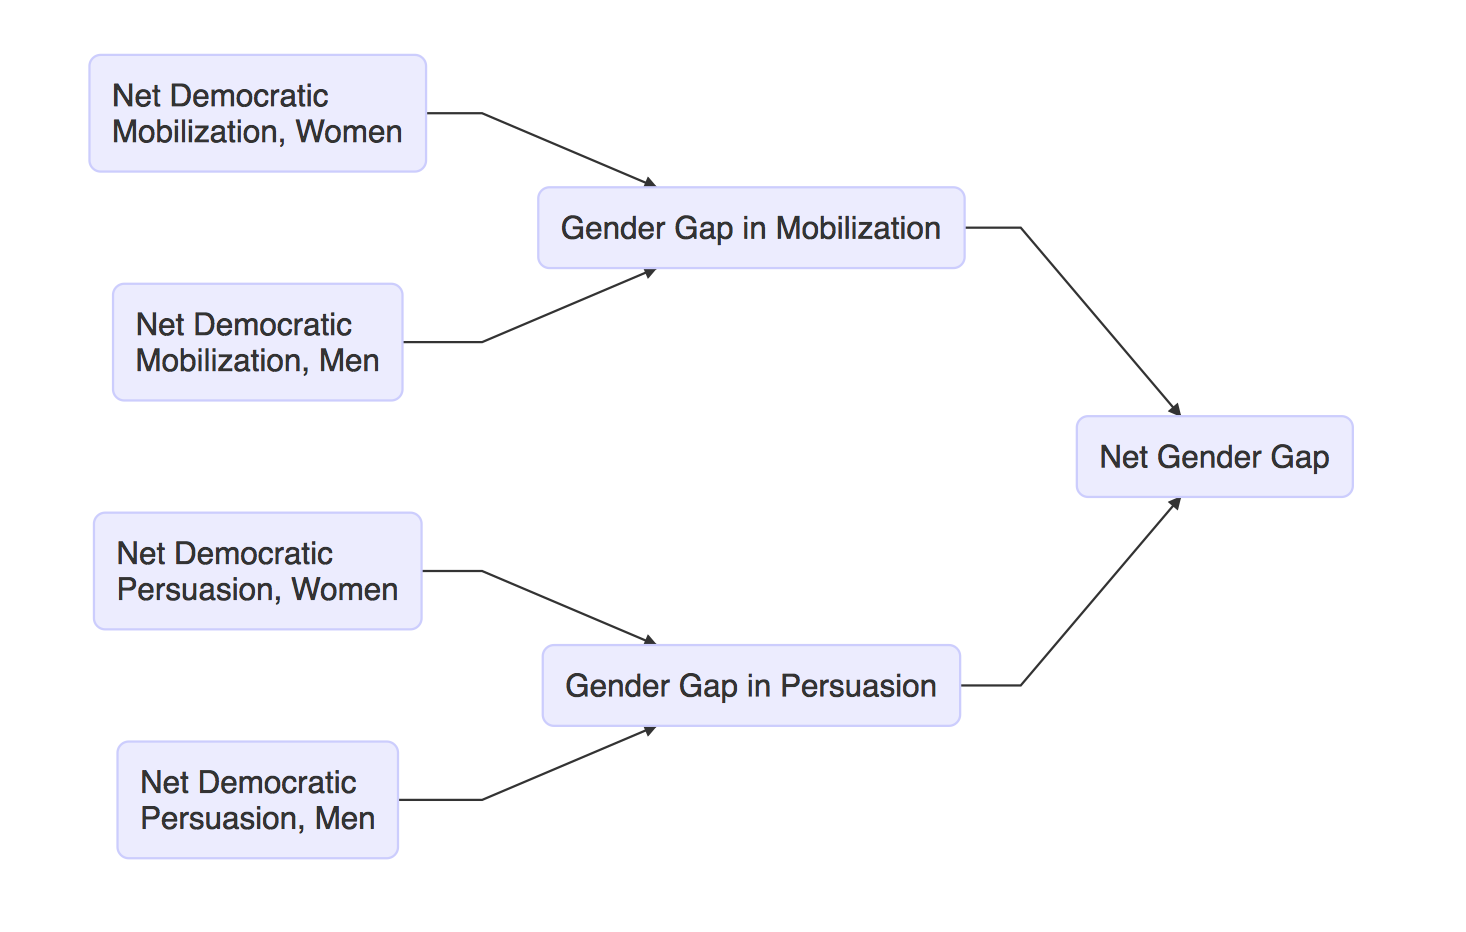
\includegraphics[width = 0.9\textwidth]{diagrams/model-gaps.png}
 % \end{center}

\begin{center}
  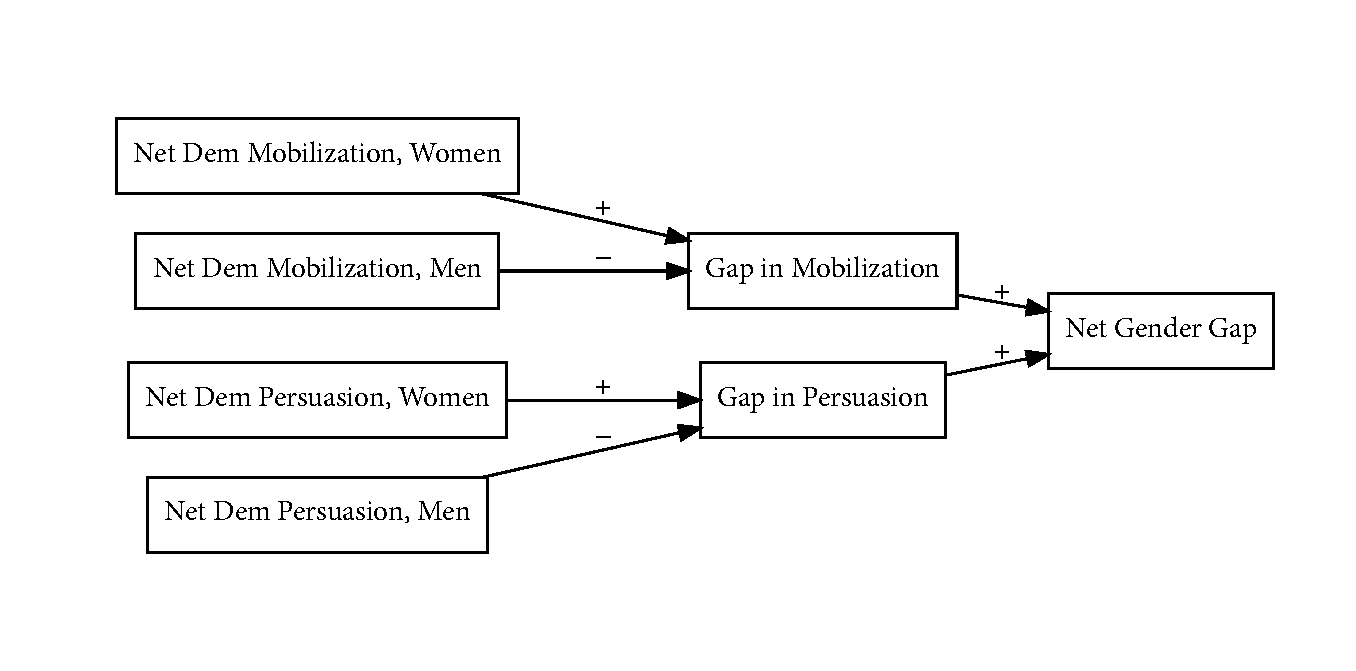
\includegraphics[width = \textwidth]{diagrams/net-gap-mechanisms.pdf}
\end{center}

% \hfill \\ % this is done to prevent squishing up to the text
%           % I should find a less-hacky fix to that
% \noindent 
% \begin{tikzpicture}
%   \matrix (m) [matrix of math nodes,
%                row sep = 1em, column sep = 4em, minimum width = 2em] {
%   \text{Net Dem Mobilization, Women} \\
%   & \text{Gap in Mobilization} \\
%   \text{Net Dem Mobilization, Men} \\
%   & & \text{Net Gender Gap} \\
%   \text{Net Dem Persuasion, Women} \\
%   & \text{Gap in Persuasion} \\
%   \text{Net Dem Persuasion, Men} \\
%   };
%   \path[-latex]
%     (m-1-1.east) edge node [above] {+} (m-2-2)
%     (m-3-1.east) edge node [above] {-} (m-2-2)
%     (m-5-1.east) edge node [above] {+} (m-6-2)
%     (m-7-1.east) edge node [above] {-} (m-6-2)
%     (m-2-2.east) edge node [above] {+} (m-4-3)
%     (m-6-2.east) edge node [above] {+} (m-4-3)
%       ;
% \end{tikzpicture}

% advantages: 
% net votes = sum of net mechanism advantages
% broken down by gender: net gender gap
% so the net gap = sum of mechanism gaps
% all related by 1-to-1 magnitude



%In summary, our theory describes how election outcomes are the result of simple building blocks: the mobilization and persuasion of men and women voters. We use this approach to conceptualize the net gender gap and the net Democratic vote as functions of the same set of terms---the Democratic party's \emph{net advantage} in each mechanism in each gender---rearranged in slightly different ways. We operationalize these terms in the following section, and then we trace how gender differences in each mechanism affect the overall gender gap and election outcome. 


\begin{comment}
Not sure that we ever have directly explored a measure that would be positive if the Democrats net more votes from women (over men) than the Republicans net from men (over women). Net gender gap is $(DW - RW) - (DM - RM)$. This other measure would be $(DW - DM) - (RM - RW)$

MGD: if you distribute that out, it would actually be equivalent to the net Democratic vote. Which is to say: ``if the Democrats net more votes from women over men than Republicans net from men over women, Democrats win the election.'' It's almost tautological but maybe what it actually shows is the need to compare any election to a past baseline. When the electorate changes in *some such way* its affect on the gender gap is X and its affect on the election outcome is Y. 
\end{comment}


\begin{comment}
%
 \begin{center}
  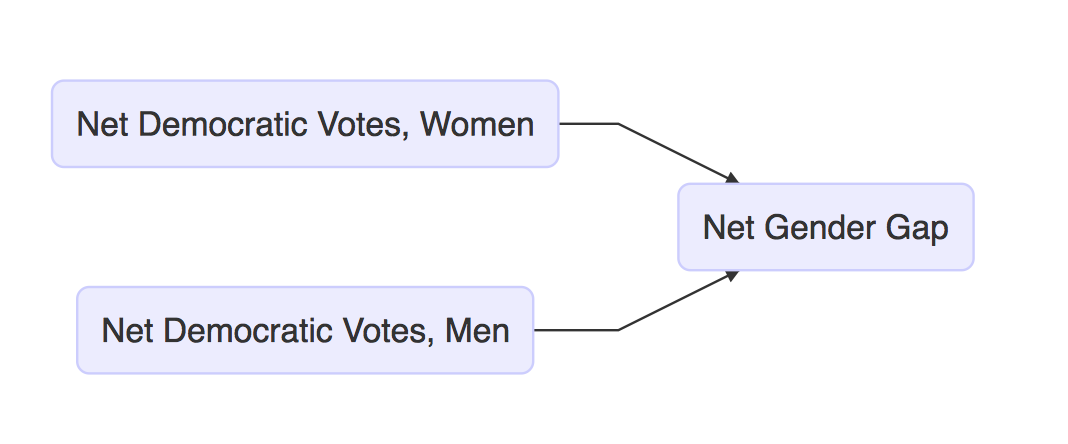
\includegraphics[width = 0.6\textwidth]{diagrams/net-gender-gap.png}
 \end{center}
\end{comment} 

\begin{comment}
%
 \begin{center}
  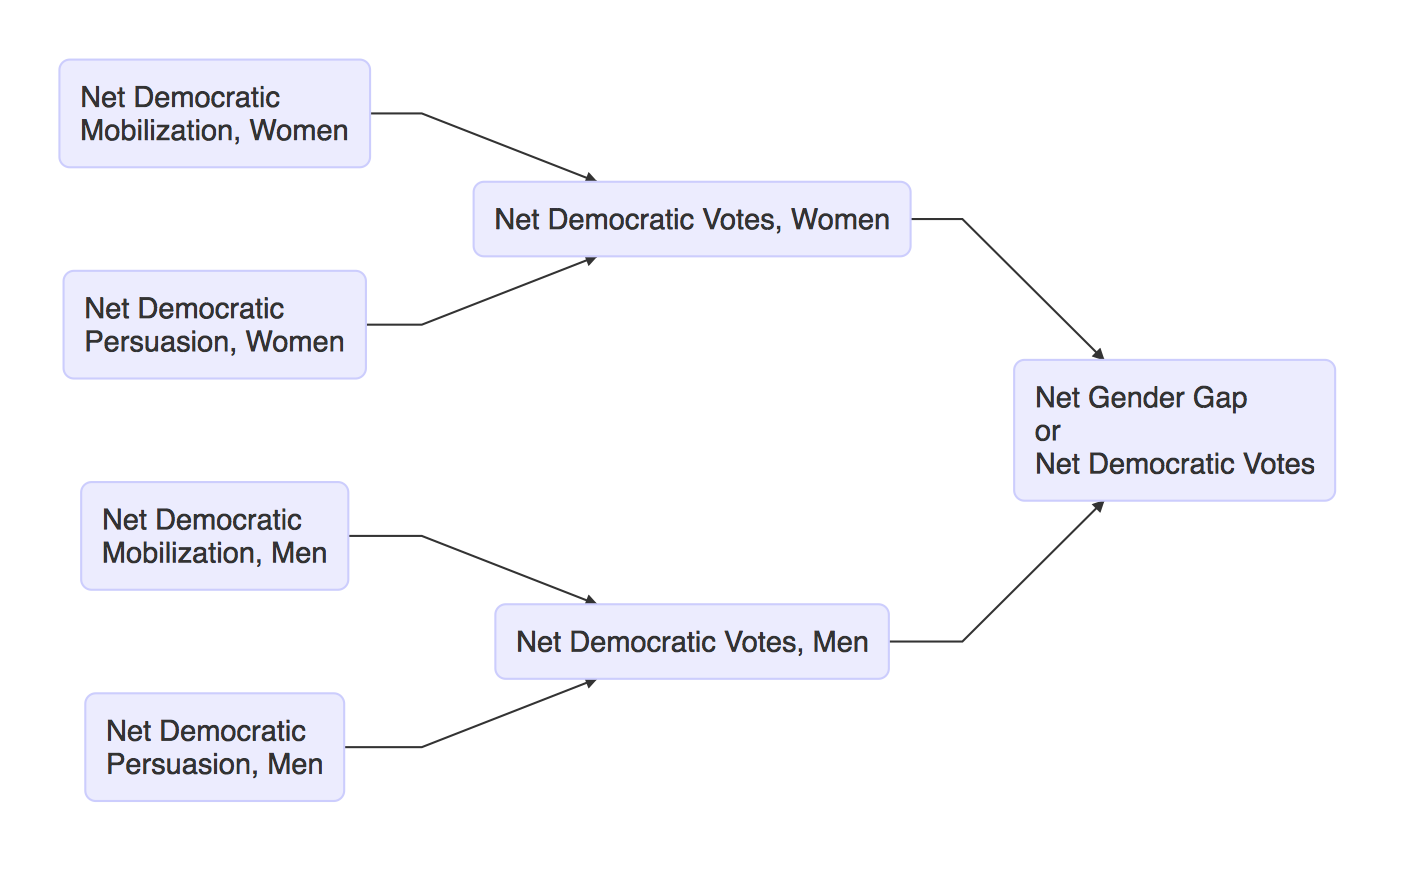
\includegraphics[width = 0.9\textwidth]{diagrams/model-votes.png}
 \end{center}
%
\end{comment}





\section*{Measuring Mobilization and Persuasion}


To operationalize our stylized model of election outcomes, we lay out a measurement strategy that models the electoral behavior of men and women as partisan attachments that become votes through mobilization and persuasion. Final vote totals must also include votes from independents and other individuals not affiliated with either major party. This section describes how we specify our model using real data.

Stated more formally, our proposition about mobilization and persuasion is that the number of votes for party $p$ from gender $g$ in election cycle $t$ begins with the number of individuals identifying with the party, plus a function that describes how partisanship is transformed into the number of votes,
% 
  \begin{align}
    \mathrm{Votes}_{pgt}  &=  \mathrm{Partisans}_{pgt} + f(\cdot)_{pgt}
  \end{align}
% 
where $p \in \{D, \, R\}$ represents Democrats and Republicans, and $g \in \{M, \, W\}$ represents men and women. To specify the filtering process, we add terms to represent mobilization and persuasion, plus an additional term to capture the remaining votes that party $p$ earns from voters not affiliated with either major party, such as independents and third-party identifiers. Equation~\ref{eq:the-model-pgt} specifies this decomposition of the vote, which forms the basis of several useful quantities in the analysis.
 \begin{align}
  \label{eq:the-model-pgt}
  \mathrm{Votes}_{pgt} &= 
   \mathrm{Partisans}_{pgt} + \mathrm{Mobilization}_{pgt} + \mathrm{Persuasion}_{pgt} + \mathrm{Unaffiliated}_{pgt}
 \end{align}

To measure baseline partisanship, we begin by collapsing the party ID index in the ANES to code every respondent as either a Democratic identifier, a Republican identifier, or unaffiliated with any major party.%
  \footnote{Missing responses for partisanship are dropped from the analysis.}
From this collapsed coding, the $\mathit{Partisans}_{pgt}$ term is simply the number of respondents of each gender in each year who identify either as Republican (for $p = R$) or Democrat (for $p = D$). Our results are not greatly affected by whether we treat leaning independents as partisans or as independents \citep{keith1992myth,miller1996new,petrocik_measuring_2009,klar2016independent}. To streamline the presentation, we show results where leaners are coded as partisans, and we place results for both assumptions in the appendix.

To measure mobilization, we code all individuals as casting a Republican vote, casting a Democratic vote, or something else.%
  \footnote{We collapse third-party votes, write-ins, and abstention from voting into one category.}
%
We define a mobilized voter as a partisan identifier who casts a party-loyal vote. The $\mathit{Mobilization}_{pgt}$ term in the equation, however, is defined in the negative as the \emph{subtraction} of non-loyal partisans. We do this in order for $\mathit{Partisans}_{pgt} + \mathit{Mobilization}_{pgt}$ to capture the number of mobilized voters. For example, if we have a group of $100$ Republican-identifying women, $70$ of whom are mobilized to cast party-loyal votes, we would express $\mathit{Partisans} + \mathit{Mobilization}$ as $100 - 30 = 70$. This formulation allows us to unpack party loyal voting into the separate processes of partisanship and mobilization.

The final two terms are straightforward. To measure $\mathit{Persuasion}_{pgt}$, we count the number of votes party $p$ receives from supporters of the other party. The $\mathit{Unaffiliated}_{pgt}$ term is all votes for party $p$ from voters who identify as neither Democrats nor Republicans.

With partisanship, mobilization, persuasion, and unaffiliated voters defined in this way, the workhorse model presented in Equation~\ref{eq:the-model-pgt} is an accounting identity that exactly defines the number of ANES respondents from each gender who vote for each major party.%
  \footnote{For the purposes of describing the model, we temporarily treat the data from ANES respondents as fixed. The analysis estimates these quantities with uncertainty.} 
Because the model is made only of simple addition and subtraction, these quantities are all on the same scale and thus can be rearranged to decompose the net Democratic vote and the net gender gap into the mechanisms at the heart of our theory. Using $p \in \{D, \, R\}$ to represent Democrats and Republicans and $g \in \{M, \, W\}$ to represent men and women, we calculate net Democratic votes and the net gender gap in each election $t$ as follows. We suppress the subscript $t$ for simplicity.
  \begin{align}
    \label{eq:net-dem-votes} % net dem votes
    %
    \mathrm{Net \, Democratic \, Votes} 
      &= \big( \mathrm{Votes}_{\mathit{DW}} + 
               \mathrm{Votes}_{\mathit{DM}}
         \big) 
      - \big( \mathrm{Votes}_{\mathit{RW}} +
              \mathrm{Votes}_{\mathit{RM}} 
        \big), \\
    \label{eq:net-gap} % net gap
    \mathrm{Net \, Gender \, Gap}
      &= \big( \mathrm{Votes}_{\mathit{DW}} - 
               \mathrm{Votes}_{\mathit{RW}} 
         \big)
      - \big( \mathrm{Votes}_{\mathit{DM}} - 
              \mathrm{Votes}_{\mathit{RM}} 
        \big),
  \end{align}
%
where each $\mathit{Votes}_{pg}$ term is itself the sum of partisanship, mobilization, persuasion, and unaffiliated voters (Equation~\ref{eq:the-model-pgt}). If both women and men vote equally in favor of the Democratic ticket, the net Democratic vote would be positive, while the net gender gap would be zero.

\begin{comment}
%
\begin{align}
\label{eq:vote-net-mechanisms} 
\begin{split}
 \mathit{Net \, Democratic \, Votes}
 &= \sum\limits_{g} \left(\mathit{Votes_{Dgt}} \right) - \sum\limits_{g} \left( \mathit{Votes}_{Rgt} \right) \\ 
 &=
  \mathit{Net \, Democratic \, Partisans} 
  + \mathit{Net \, Democratic \, Mobilization} \\
 &\quad
  + \mathit{Net \, Democratic \, Persuasion} 
  + \mathit{Net \, Democratic \, Unaffiliated}.
\end{split}
\end{align}
%
\end{comment}

As described above, a benefit of our theory is the decomposition of the net Democratic vote and the net gender gap into the Democratic Party's \emph{net advantage} over the Republican Party in each mechanism leading to the vote. The net Democratic advantage in each mechanism can be obtained by differencing Equation~\ref{eq:the-model-pgt} for Democrats minus Republicans (holding gender and time constant). Expressed using net Democratic advantage, the net Democratic vote is therefore the sum of the net Democratic votes for women plus men, and the net gender gap is the net Democratic vote among women minus the net Democratic vote among men.
%
\begin{align}
  \mathrm{Net \, Democratic \, Votes} 
    &= \mathrm{Net \, Democratic \, Votes}_{W} + 
       \mathrm{Net \, Democratic \, Votes}_{M} \\
  \mathrm{Net \, Gender \, Gap} 
    &= \mathrm{Net \, Democratic \, Votes}_{W} - 
       \mathrm{Net \, Democratic \, Votes}_{M}
\end{align}
%
The net Democratic vote for each gender, in turn, is the sum of the mechanisms that translate partisanship into votes.
\begin{align}
  \label{eq:vote-net-mechanisms-women} 
  \begin{split}
    \mathrm{Net \, Dem \, Votes}_{W} 
    &= \mathrm{Net \, Dem \, Partisans}_{W} + 
       \mathrm{Net \, Dem \, Mobilization}_{W} \\
       &\quad + \mathrm{Net \, Dem \, Persuasion}_{W} 
              + \mathrm{Net \, Dem \, Unaffiliated}_{W}
  \end{split} \\
  %
  \label{eq:vote-net-mechanisms-men} 
  \begin{split}
    \mathrm{Net \, Dem \, Votes}_{M} 
    &= \mathrm{Net \, Dem \, Partisans}_{M} + 
       \mathrm{Net \, Dem \, Mobilization}_{M} \\
       &\quad + \mathrm{Net \, Dem \, Persuasion}_{M} 
              + \mathrm{Net \, Dem \, Unaffiliated}_{M}
  \end{split}
\end{align}
The gender gap in each separate mechanism is the net advantage in each mechanism among women, minus the net advantage among men (Equation~\ref{eq:vote-net-mechanisms-women} minus Equation~\ref{eq:vote-net-mechanisms-men}). Similarly, each mechanism's contribution to the net Democratic vote is calculated by summing the two equations. 

Before turning to our analysis, we address one final methdological issue: comparability over time. We operationalize the terms in this analysis by simply counting the number of survey respondents who fall into various categories, but how do we compare these quantities across election years when each ANES survey has a different sample size? We apply a simple normalization to place these surveys on a common scale, dividing the original model in Equation~\ref{eq:the-model-pgt} by the total number of voting-eligible respondents in each survey year.%
  \footnote{We operationalize ``voting-eligible respondents'' as all individuals with valid responses to partisanship, gender, and vote outcome items.}
We choose this denominator because it is the only common denominator that includes the total number of voters and nonvoters from each partisan group from each gender. After normalizing, each term represents \emph{the proportion of the total electorate} that contributes to a party's vote share through each mechanism. This normalization is appealing for our purposes because we aim to compare partisanship among voters and nonvoters, the voting and abstention decisions of partisans, and the choices of non-partisan voters on the same scale.%
  \footnote{These proportions and their uncertainty could be estimated using a number of methods. Because each term is a proportion of the total electorate, we estimate these proportions directly using a multinomial outcome approach. We code ANES respondents along an 18-category variable that exhaustively indexes all combinations of gender (men and women), partisanship (Democrat, Republican, unaffiliated), and vote choice (Democrat, Republican, and ``other''), and then we estimate the proportion of the electorate in each category by modeling the number of respondents in each category as a multinomial variable. This routine gives us estimates of all 18 probabilities under the constraint that they sum to 1. We use Markov chain Monte Carlo to estimate the uncertainty in these probabilities and propagate uncertainty through each of the above equations. We view this estimation routine as non-essential to the rest of our approach; other researchers may use different approaches to incorporate statistical uncertainty into a similar analysis. More information about this routine can be found in the appendix.}


\section*{How Mobilization and Persuasion Shape Elections}

Having outlined our theoretical and methodological approaches, we are now prepared to describe how these mechanisms connect the gender gap to the vote. Figure~\ref{fig:RHS-simple} displays our measures of partisanship, mobilization, persuasion, and unaffiliated voters for presidential elections from 1952 to 2012. Because these trends are plotted after normalization, the vertical axis represents each quantity as a percentage of all voting-eligible citizens. Each column displays the various right-hand side terms of Equation~\ref{eq:the-model-pgt}. The one exception is column~2, which shows the share of mobilized voters $\big(\mathit{Partisanship}_{pgt} + \mathit{Mobilization}_{pgt}\big)$ rather than the stand-alone $\mathit{Mobilization}_{pgt}$ term, which would be a negative number as described above. Solid points represent women, and hollow points represent men. Colors indicate the party that benefits from each source of votes; for example, the red lines in the ``Persuasion'' panel represent Republican votes obtained from Democratic partisans. As noted above, we present results where leaners are coded as partisans voters, but the appendix contains results with the opposite assumption.

% \todo[inline]{rows for men and women?}

\begin{figure}[hbt]
  \centering
  \caption{Measures of Mobilization, Persuasion, and Voting by the Unaffiliated 1952-2012}
  \includegraphics[width=\textwidth]{graphics/mc-rhs.pdf}
  \label{fig:RHS-simple}
  \notes{For presentational purposes, Column 2 displays the share of mobilized voters instead of the $\mathit{Mobilization}_{pgt}$ term from the model equation. The share of mobilized voters is the share of partisans minus the share of non-mobilized partisans. Leaning independents are coded as partisans.}
\end{figure}


This figure captures important findings from the study of U.S.\ elections, thus offering some validation for our measurement strategy. Looking at the first panel, we recover similar trends in partisanship as \citet{kaufmann1999changing} and \citet{norrander1997independence}; a long-standing partisan advantage for the Democratic Party in the aggregate, with a dramatic decline in Democratic identification and increase in Republican identification among men from the 1960s through the 1980s. Partisanship among women has fluctuated in the short-term but is generally stable around long-term averages, with Democratic-identifying women making up 25 to 30 percent of the electorate since the 1970s, and Republican women making up around 20 percent.

Trends in the share of mobilized voters (the second panel) are also consistent with prior scholarship (e.g., \citealt{flanigan2015}). Although Democrats have historically outnumbered Republicans in party identification alone, lower levels of turnout among Democratic partisans results in two parties that mobilize a similar number of voters over time. Party-loyal voting among Democrats steadily increased since its low points in the late 1960s and early 1970s. Party-loyal Democratic women was always a large group in the electorate, but they grew from less than 15 percent of the total electorate in 1972 to more than 20 percent in 2016. The increase in Democratic votes from party-loyal men saw a similar rise, from under 10 percent of the electorate in 1972 to about 15 percent in 2016. Turnout among Republicans fluctuates in response to short-term electoral contexts---higher in the 1970s and '80s and dropping in the 1990s---but the trends for men and women are quite similar to one another.

Moving to the third panel, trends in persuasion are also consistent with past scholarship. Republican candidates in past decades consistently collected more swing votes from Democratic identifiers than Democratic candidates have from Republican identifiers. The only years in which Democrats appear to numerically outperform Republicans in swing voting are 1964 and 1996, two strong Democratic years. Taken together, these trends in mobilization and persuasion are broadly consistent with the ``two majorities'' interpretation of this period in American politics, where Democrats formed a partisan majority which Republicans often overcame in turnout and vote choice \citep{claggettshafer1995twomajorities}. In more recent decades, both parties collect more votes through mobilization and fewer through persuasion, reflecting heightened party loyalty in the current era of party sorting and polarization.

Lastly, the number of votes obtained through unaffiliated voters is generally small but mirrors the partisan swing of presidential elections, giving more votes to Republicans for the campaigns of Presidents Eisenhower, Nixon, and Reagan, and swinging to Democrats for the campaigns of Presidents Johnson and Clinton (1992) especially.



\subsection*{Sources of the Gender Gap}

Using these new measures of partisanship, mobilization, persuasion, and party-unaffiliated voting, we compute gender differences in the partisan impact of each trend to trace how each mechanism contributes to the net gender gap. To do this, we first calculate the Democratic advantage in each mechanism separately for women and men (Equations~\ref{eq:vote-net-mechanisms-women} and~\ref{eq:vote-net-mechanisms-men}). For example, there is a Democratic advantage in partisanship among women if a greater number of women identify as Democrats than as Republicans. We then get the gender gap in each mechanism by differencing the Democratic advantage among women minus the net advantage among men. A gender gap in a given mechanism arises if the Democratic advantage among women is greater than the Democratic advantage among men. If the numerical impact of women's and men's behavior is equivalent (men and women are equally pro-Democratic or pro-Republican), the gender gap in a given mechanism is zero. Democratic advantages and gender gaps are calculated after normalization and thus are expressed as proportions of the overall electorate. 

In Figure~\ref{fig:partials-on-gap}, we decompose the net gender gap into the separate mechanisms of partisanship, mobilization, persuasion, and votes from unaffiliated individuals. The first four panels of the figure present the data for these separate mechanisms over time. On the vertical axis we plot the partial effect of women's and men's behavior on the gender gap. For example, if the Democratic advantage among women in a given mechanism is positive, this exerts a positive partial impact on the gender gap, and will be shown as positive values on the graph. For men, the relationship between Democratic advantage and the gender gap is the opposite; the gender gap grows if men vote more \emph{Republican}, so a Democratic advantage among men exerts a negative impact on the gender gap and is represented by negative values in the figure. 

We then plot the gender gap in each mechanism as a dark, solid line with a 95 percent uncertainty interval.%
  \footnote{Because we generate uncertainty intervals using MCMC, we have a distribution for each estimated value. The thick trend lines represent the mean of each distribution, and intervals represent the inner 95 percent of the distribution.} 
The gender gap in each mechanism is positive if the Democratic advantage among women is greater than the Democratic advantage among men. If men and women exert the same numerical impact on the election in their partisanship, mobilization, and so on, the trends for men and women would be perfect reflections of each other across the horizontal axis, and the gender gap in each mechanism would be zero. The \emph{net} gender gap, plotted in the final panel, is the sum of the gender gap in each mechanism. We again point out that all of the values in this figure are simply differences in proportions calculated from raw ANES data.


% \todo[inline]{I've been wondering about how to ``formalize'' our findings. We present graphics and some intuitive description of them, but no guideline for how to use our method to come to formal conclusions in situations where the trends are not obvious. Should we be thinking about this? (Should there be another paper where we apply this to more Axelrodian groups?) Might be helpful to include tables where we quantity the contribution of each mechanism to the gap, to numerically show how the growth in one mechanism might be offset by some other mechanism. Variance decomposition of the change in each sub-trend? E.g. from 1956 to 1960, women's partisanship changes by x percent, men's partisanship changes by y percent, so the fraction of absolute variance in partisanship explained by women is sqrt($x^{2}$)/sqrt($y^{2}$), which could be calculated for every mechanism and then plotted over time to determine, formally, which mechanisms are ``most responsible'' for trends in the GG and in the Dvote. Is partisanship the ``largest influence'' on the gender gap over time? Is mobilization and persuasion the ``largest influence'' on the growing Democratic vote over time? Seems like these could be formalized. I'm imagining a plot that shows the distribution of estimated variances explained}


% \begin{figure}[hbt]
\begin{sidewaysfigure}[p]
  \centering
  \caption{How Each Mechanism Affects the Gender Gap}
  \label{fig:partials-on-gap}
  \includegraphics[width = \textwidth]{graphics/mc-gap-partials.pdf}
  \notes{Democratic advantage among women exerts a positive effect on the net gender gap, while Democratic advantage among men exerts a negative effect. Women are shown with solid points, men with hollow points. The thick line indicates the gender gap in each mechanism. The right-most panel is the sum of the net gender gap across all mechanisms.}
\end{sidewaysfigure}
% \end{figure}

Beginning with the left-most panel, we find that the Democratic advantage in partisanship among men and women had an offsetting influence on the gender gap in the earliest elections covered by the ANES data (i.e., the gender gap in partisanship is near zero). Consistent with previous research, the Democrats' advantage in men's partisanship decreased in the 1970s and 1980s, creating a gap in partisanship that persists through the remainder of the time series. Although we use the same data as classic studies of the development and evolution of the gender gap \citep{kaufmann1999changing,norrander1997independence,norrander1999evolution}, our approach affords us three important findings about the nature of the gender gap in voting. First, we find that the gender gap in partisanship much emerges earlier in the series than the gender gap in voting (contrary to \citealt{kaufmann1999changing}, although see \citealt{gillionetal}). Although there are idiosyncratic gender differences in voting in the early half of the series (such as in 1964, see also \citealt{norrander1999evolution}), the stable and persistent gender gap in voting as we understand it today emerged in 1980. We find that a gender gap in partisanship appeared more than a decade earlier in the elections of 1964 and 1968, roughly equal in size to the net gender gap in voting (about five percent of the total electorate).%
  \footnote{Although five percent seems like a small gap, it is important to remember that our measurement approach uses a larger denominator than the conventional gender gap measure (the total electorate versus only major-party voters) to compare all mechanisms among all groups on the same scale.}
Second, our approach underscores how recent variation in the partisan gender gap is almost entirely driven by variation in women's partisanship. While we acknowledge other scholars for observing that women's partisanship grew more influential in the 1990s \citep{box2004dynamics,kaufmann2002culture}, our measurement approach emphasizes how the gender gap in partisanship since the 1990s is a near-perfect reflection of the variation in women's partisan attachments. And third, as a quick visual comparison between the first panel and the remaining panels show, partisanship is a much larger influence on the gender gap than mobilization and persuasion are.

The second panel of Figure~\ref{fig:partials-on-gap} plots the data on the gender gap in mobilization. In our mathematical approach, mobilization is operationalized as the \emph{loss} of partisan identifiers in the turnout process. A Democratic advantage in mobilization forms, therefore, when Democrats lose fewer votes from their supporters than Republicans lose from theirs. As it happens, Republicans are advantaged in mobilization throughout the entire series---Democrats have a long-running advantage over Republicans in partisanship, but they have a long-running disadvantage in turning those partisans into voters. The figure shows this pattern among both men and women. Not only is the Democratic advantage in mobilization negative in the aggregate, the overall effect of mobilization on the net gender gap is negative as well. This indicates that Democrats' losses among women are greater than their losses among men. In recent years of partisan polarization, the Republican advantage in mobilization has shrunk dramatically, but mobilization nonetheless produces a slight negative gender gap even in the most recent 2016 data. 

The third panel of Figure~\ref{fig:partials-on-gap} shows the gender gap in persuasion. As with mobilization, Republicans tend to be the numerical beneficiaries of swing voting. This is shown by the negative values for women and positive values for men---pro-Republican behavior among women decreases the gender gap, while pro-Republican behavior among men increases it. Also like mobilization, the long-term advantage for Republicans shrank over time, nearly disappearing in election years since 2000. Unlike mobilization, however, the Republican advantage in persuasion had a very small impact on the gender gap, which is negative in most years but with a gap of zero contained within the 95 percent interval. In short, Republicans generally outperform Democrats in persuasion, but their advantage is similar for among men and women.

Taking our data from partisanship and mobilization together, we can see how the earliest gender gap in partisanship failed to appear in voting. Although the gender gap in party ID emerged as early as 1964, the majority of the gap was offset by a pronounced, negative gender gap in mobilization that was statistically significant for the majority of elections throughout the time series. Researchers have long understood that Republicans have higher turnout and party loyalty than Democrats on average; our analysis shows how this pattern falls unequally among women and men, suppressing a gender gap in party ID from appearing in the final vote for more than a decade.

The final mechanism in our model is the votes of unaffiliated citizens, which we plot in the fourth panel of Figure~\ref{fig:partials-on-gap}. Because unaffiliated voters usually reflect the patterns in swing voting among partisan identifiers, the overall impact of unaffiliated voters on the gender gap is similar to the impact of persuasion. Although a few elections stand out as having suggestive impacts on the gender gap, these moments in the time series are idiosyncratic. Pro-Republican landslides in 1972 and 1980 elicited more votes from unaffiliated men than unaffiliated women, and the 1996 election---the largest gender gap in the ANES data---was widened in part by pro-Democratic voting among unaffiliated women. But in most elections, unaffiliated men and women exert roughly equal and opposite influences on the gender gap. 

The final panel in Figure~\ref{fig:partials-on-gap} shows the net gender gap, which is the sum of the gender gap in each mechanism in our model. This trend captures the common understanding of the gender gap as emerging in the 1980s and persisting mostly unchanged in the years since (1996 being a blip from the otherwise constant trend). We emphasize that our measure of the \emph{net gender gap} shows a similar pattern to the conventional gender gap only because men and women are nearly equal in voting power. If we applied our analytical method to differently sized groups (such as racial groups), our net gap measure would differ greatly from the conventional measurement approach.




\subsection*{Gender Gaps and the Formation of the Democratic Vote}

Our theoretical framework is designed to show how the gender gap and the Democratic vote are composed from the same building blocks. Now that we have decomposed the gender gap into partisanship, mobilization, persuasion, and unaffiliated voters, we show these forces aggregate into the final election outcome.

Figure~\ref{fig:partials-on-vote} shows how the Democratic advantage in each mechanism affects the net Democratic vote, with separate trends for men and women. Positive values indicate a net Democratic advantage and, in turn, a positive influence on the net Democratic vote. A Democratic advantage among women both widens the gender gap and increases the Democratic vote, but a Democratic advantage among men would decrease the gender gap even as it increases the Democratic vote. A positive gender gap forms when the Democratic advantage in one mechanism is greater for women than it is for men---the size of the gender gap can be interpreted as the space between the trend lines for women and men. As with the previous figure, the first four panels plot the Democratic advantage in partisanship, mobilization, persuasion, and unaffiliated voters. The final panel shows the net Democratic vote among men and women, which is the sum of the four preceding mechanisms. All values reflect normalization and are expressed as a percentage of the eligible electorate. 

  \begin{sidewaysfigure}[p]
   \centering
   \caption{Relating the Gender Gap and the Election Outcome: Gender differences in the sources of Democratic votes}
   \label{fig:partials-on-vote}
   \includegraphics[width=\textwidth]{graphics/mc-vote-partials.pdf}
   \notes{Women are shown with orange solid points, men with hollow green points.  The right-most panel is the Net Democratic Vote for each gender, summing across mechanisms.}
  \end{sidewaysfigure}

The left-most panel plots the Democratic advantage in partisanship for men and women. As before, we observe that a gender gap in partisanship emerges as early as the 1960s and widens as the Democratic advantage dissipates more quickly among men than among women.%
  \footnote{We show in the appendix that when leaners are coded as unaffiliated, the Democrats' partisan advantage among women decreases somewhat as well. This is driven by an increasing tendency of Democratic-leaning women to identify as independents, but not as Republicans. This is one area where the coding of leaners has slight bearing on the findings, but the dominant interpretation holds: change among men is the primary driver of the partisanship gap.}
By 1988, the trend among men flattens, and variation in the gender gap is driven primarily by women's partisanship. But the variation among women is much more volatile than the definitive and permanent shift among men's partisanship. If we link the effects on the gender gap to the effects on the Democratic vote, trends in partisanship contradict the conventional wisdom of gender gap punditry. If the gender gap in party ID was created by a sharp and enduring erosion of Democratic partisanship among men, then the primary driver of the gender gap has decreased the net Democratic vote.

The second panel shows how the Democrats' advantage in partisanship is transformed by differential mobilization. As discussed above, a negative gender gap in mobilization counteracted the gender gap in partisanship in its earliest years, preventing the net gender gap from emerging until 1980. We see this negative gap in Figure~\ref{fig:partials-on-vote} as well, but the Democratic disadvantage in mobilization is much more apparent here. As much as the Democratic Party enjoyed an advantage in partisanship, it lost almost all of that advantage by failing to turn out its voters. As the time series progresses, Democrats dramatically improve their mobilization efforts, but that improvement does not greatly affect the difference between men's and women's mobilization. Data from 2016 suggest that even though Democratic women are a large group in the electorate, Democrats' lose more women through mobilization than Republicans do, so the negative gender gap in mobilization remains. In sum, the evidence from mobilization contradicts the conventional wisdom as well. Democratic gains in mobilization do not come disproportionately from women, and Republicans still have an edge on Democrats when it comes to mobilizing party-loyal women.

Turning to the middle panel of Figure~\ref{fig:partials-on-vote}, we see the effect of persuasion over time. Republicans were the historical beneficiaries of persuasion, as shown by the largely negative values in the plot, but the trends are essentially identical for men and women. As far as the conventional wisdom regarding the relationship between the gender gap and the Democratic vote is concerned, persuasion tells a similar story as mobilization: Democrats have benefited in recent years by \emph{preventing} defection among their own ranks, but this benefit does not depend more heavily on women than on men. Moreover, we find no evidence that Democrats' recent messaging about the Republican ``war on women'' has a noticeable effect on the balance of crossover voting among women.
% ^ I was able to salvage a point about the persuadability of women after all (MGD)

Moving to the fourth panel, the vote choices of unaffiliated citizens appear to display few gender differences or trends over time; unaffiliated men and women shift their votes in response to specific election contexts in very similar ways. Moreover, these shifts have a minuscule topline impact when compared to group differences in party affiliation, mobilization, and persuasion. If the voting behavior of unaffiliated men and women diverged, those diverges were brief and idiosyncratic, indicative of no broader trend. 

The final panel displays the net Democratic vote for women and men, which is the sum of the four preceding panels. The early half of the time series fluctuates wildly between landslide elections in 1964, 1972, and 1984. By the latter half of the time series, stabilization in the preceding mechanisms leads to a more stable trend in the net Democratic vote. Men are almost equally divided in voting for the two parties, while women are decidedly Democratic. This is consistent with the high-level finding from Figure~\ref{fig:topline} that the gender gap weakly coincides with higher Democratic vote shares---both have increased in recent decades. But our examination of the various mechanisms that produce the vote suggests that the relationship between the gap and the overall vote is spurious in a specific way. The forces that boost the Democratic vote share in recent elections (Democrats stemming their losses in mobilization and persuasion) are not the same forces that cause the votes of men and women to diverge (partisan change among men).

Decomposing the vote in this way underscores our two primary arguments about the link between the gender gap and the Democratic vote. First, there is no necessary relationship between the gender gap and the Democratic vote share. While both the gap and the vote can be theoretically understood as partisanship attachments that are transformed by mobilization, persuasion, and unaffiliated voters, the long-term electoral trends that impact these series have the potential to be reinforcing, counteracting, or somewhere in between. And second, while there is no necessary relationship between the gap and the vote, there is a contingent relationship that runs counter to the conventional wisdom. The primary driver of the gender gap---changing partisanship among men especially---has unfolded to the benefit of Republicans rather than Democrats. Meanwhile, the causes of increased Democratic voting over the same time period---shrinking Republican advantages in mobilization and persuasion---have unfolded in a comparatively gender-neutral fashion.



% ---  -----------------------




% Key: early gap in PID (-) gets suppressed by mobilization (double --)

% as time goes on, negative mobilization gap decreases. This increases the gender gap and the Democratic vote (+)

% Persuasion overall decreases (+) but relatively small impact on gender gap. 

% Idiosyncratic influences from Unaffiliated voters have mixed effects. 

% Today: forces are in an interesting balance. Partisan advantage among women (+/+) but slight disadvantage among mobilization w/ inert influence.



% \todo[inline]{Counterfactuals? Let's say the net effect of men's PID is zero: what is the gender gap, what is the vote outcome?. Multi-panel graph where we zero out each successive mechanism, and measure the difference from the actual outcome? Explicitly quantify each factor's contribution to gap and vote in each year (but how to deal with the covariance). Perhaps partial out the average year effect as well?}


% \todo[inline]{MGD note to self: still want to check dynamics to see if there is anything good}



\section*{Conclusion}

Compared to other groups in the electorate, the differences between the vote choices of men and women are slight. But even modest differences can have large impacts on election outcomes because, unlike many other groups, men and women make up large and nearly equal voting blocs. Elections results can hinge on small shifts for either group. Campaigns naturally pursue both groups openly and aggressively, although disproportionate attention in recent years has gone to the ``women's vote.'' 

In this article we have confronted the assumption that a larger gender gap works to the advantage of Democratic candidates. To better understand how the behavior of male and female votes affects elections, we developed a general theory of electoral gaps that may be applied to many sociodemographic groups in the electorate. Our framework posits that election outcomes are the result of underlying party identification in the electorate as modified by two mechanisms---the mobilization of a party's supporters and the persuasion of the other party's supporters---plus the vote choices of unaffiliated voters. There is no \emph{necessary} relationship between an electoral gap and the overall party vote share, but this is not because gender is unimportant to voting. Instead, gender may matter in different ways at each stage of the process. 

Applying this theory using survey data across 16 presidential elections, we emphasize two takeaways about the gender gap and the Democratic vote. Although there is a weak, positive relationship between the gender gap and the Democratic vote, it is a spurious relationship created by the aggregation of separate trends in partisanship, mobilization, and persuasion. When these trends are disaggregated, we find that the growing divides between men and women (driven mainly by partisanship) work to the advantage of Republicans, not Democrats. Changes in the mobilization and persuasion of party supporters has a relatively weak impact on the gender gap, but Democrats have benefited from increased turnout and reduced defection among both men and women.

We are struck that these trends appear almost to be in equilibrium, canceling out one another in the aggregate to obscure the overall effects of the gender gap on the vote. Changes in just one of them could advantage a party significantly in a particular election. With the framework provided here, it is possible for campaigns, journalists, and scholars to identify what specific long-term and short-term factors are responsible. We believe that these intriguing cross-cutting trends ultimately demonstrate the analytical utility of our endeavor to disentangle the various mechanisms that lead to vote divisions between groups. We hope that future research will draw on the methods proposed here to gain further insight into the interwoven long- and short-term causes that create group-level differences in voting.

Having built a foundation for this kind of analysis, future research may proceed in several interesting directions. An immediate extension of our analysis would decompose men and women rather than treating them as cohesive voting blocs. Dividing each gender by race, marital status, or age could illuminate how these subgroups have uniquely contributed to the gender gap and election outcomes. Because the data analysis covers six decades of elections, it would also be possible to examine debates over how much partisan realignment in the South affected the gender gap in voting (\citealt{kaufmann2006ps,norrander1999evolution,ondercin2018}). Moving outside the application to gender, researchers are also able to analyze entirely different groups in the electorate. In light of the 2016 presidential election, researchers could focus on key groups such as urban and rural voters that unlike men and women are of vastly different sizes. We believe the gender application is important because the two groups are equally matched, but the utility of our approach could be more apparent when focused on groups of much different sizes.

\begin{comment}
% This could go in the appendix.
One factor that deserves attention in subsequent research is demographic change in the electorate. The decades covered by the ANES surveys coincides with substantial social changes including women entering the paid workforce in large numbers but also growth in the nonwhite share of the electorate. Over time the nonwhite population has become more Democratic in its leanings and has turned out at higher rates to vote. Although we lack the space to fully examine these factors, we replicated our analysis after limiting the sample to non-Hispanic whites, setting aside racial and ethnic change as drivers for the patterns we observe. When we do this, we find a stronger decay in Democratic partisanship among whites than in the full electorate, especially among white women. As a result, Republicans managed to get more votes from both partisanship and mobilization of white voters, but the gender divide in partisanship was weaker. Interestingly, because the baseline trend among white women is a Republican shift (as with men), acute increases in the partisan gender gap are driven by short-lived increases in women's Democratic partisanship rather than a long-term exodus of men from the Democratic coalition. The contributions of white women are also more volatile when viewed in isolation. Thus, some of the stability of women's behavior appears to be influenced by a growing base of Democratic-leaning Hispanic and nonwhite women who counterbalance the comparatively volatile trends among relatively conservative white women. In turn, it appears that near-term campaign maneuvers and election-specific forces have more influence over the voting decisions of white women than nonwhite women.
\end{comment}








% \newpage 
\bibliographystyle{bib/apsr2006.bst}
\bibliography{bib/gender-bib.bib}

\end{document}